\chapter{Results}

\textbf{The origin of SARS-CoV-2 in Europe} 
While the first case in Europe was reported to ECDC by France authorities on January 25, the first European wave is suspected to have started earlier but been undetected, mistaken for other common repiratory diseases in winter. In our model, we assume the origin of SARS-CoV-2 in Europe to be an imported case from China to any of the European countries. We can select a single event of interest from the inferred epidemic trajectories, and summarise its time and location. To study the origin of SARS-CoV-2 in Europe, we analyze the time and destination of the first imported case and estimate the origin of the European epidemic on January 2020 ($95\%$ CCI), Figure \ref{fig:firstEU} \todo{with final results}. The actual reported date to ECDC is in the tail of the $95\%$ credible interval. As shown in Figure \ref{fig:firstEUcountry} A, we place the destination country of this first imported case in Italy or France, with x of probability each.  

\begin{figure}[h]
    \centering
    \includegraphics[width=\textwidth]{210205_europe10_figtraj01.png}
    \caption{\textbf{First case of SARS-CoV-2 in Europe.} In the histogram, we count how many of the inferred epidemic trajectories started the European epidemic each day. From these counts, we estimate the probability density of the origin in Europe (in grey). The median date is drawn with the solid vertical line, and the date of the first reported European case to ECDC with a dashed vertical line.}
    \label{fig:firstEU}
\end{figure}

Likewise, we analyze the first ten imported cases to Europe to estimate the main source of exported SARS-CoV-2 cases early on and their destination. China is the main source of these first introductions, supporting the hypothesis of the European epidemic seeded by several and not just one imported cases from China, Figure \ref{fig:firstEUcountry} B.  The role of Italy as the receptor of these first cases is highlighted even more looking at several cases. Early introductions in Spain have a very low probabilty, looking like Spain was not a key player in the origin of SARS-CoV-2 in Europe. \todo{with final results}  Figure \ref{fig:firstEUcountry} C.  

\begin{figure}[h]
    \centering
    \includegraphics[width=\textwidth]{210205_europe10_figtraj02.png}
    \caption{\textbf{First imported cases of SARS-CoV-2 to Europe.} \textbf{A} We estimate the probability distribution of the time for the first imported case to Europe (in grey). Each row highlights the probability of this first case going to the indicated country (in color). \textbf{B} In a similar way, we considered the time of the ten first imported cases into any of the European country, and plot the time probability distribution (in grey). In the rows, we plot the probability of each country being the destination country of any of the first 10 imported cases to Europe (in color). \textbf{C} Same probability distribution of the time for the 10 first imported cases to any European country (in grey) than in B, but in each row we highlight in color the 
    probability of these cases coming from a specific country.}
    \label{fig:firstEUcountry}
    \todo[inline]{ticks for every month}
\end{figure}


\textbf{The early spread of SARS-CoV-2 among the European countries}


Since in our model we consider the different European countries, we can also estimate from the infered epidemic trajectories the origin of the epidedmic in each particular country. In Figure we have the origin time for each country compared to the ddate of the first reporrted case to ECDC by that country. In average, we predict a delay in detection of x days for the Eurropean countries, out of the $95\% CCI$ for France, Germany and Italy. Origin in Spain close to the official detection day. We estimate that the epidemic in any of the European countries was seeded by an imported case from China as seen in Figurem with some small prrobability for Germany and Italy of having orriginatetdd from a case from each other, and mostly half of the rpobability in the case of Spain from the epidemdic started with a case imported from one of the others Euroopean countries. Same than before, we can look to the first 10 imported cases to each country and now we see that the transmission between european countries adquire much moer importance,  so once SARS-CoV-2 entered Europe, the transmission between european countrries were soon more important than the cases coming from China. This could relate also to the decrease in tthe trravel to and from China seen in figure.

Among the European countries, France and Germany have the earlier time of introduction, followed by Italy, Other European deme and Spain. We can compare this inferred dates of introduction with the day each country reported its first case to ECDC. In all cases, the reported day was later than the median of the inferred distribution, but it is inside the 95\% interval.\\

The first case in each European country could have been imported from China or from other European country with an ongoing epidemic that started earlier. However, in our analysis we obtain a much higher support for China being the most probable source of the first case for all European demes, Figure \ref{fig:first} C.\\

\begin{figure}[h]
    \centering
    \includegraphics[width=\textwidth]{210205_europe10_figtraj03.png}
    \caption{\textbf{Country-level origin of SARS-CoV-2 epidemic.} For China, we consider the origin of the epidemic as the first local case while for the European countries we select the first imported case into the country. \textbf{A} We estimate the probability distribution of the date for the first case in each of the locations included in the analysis (in grey). We highlight the conditional probability for the source of the first case in each country (in color).  \textbf{B} The ten first imported cases into the country are selected, and we estimate the probability distribution of their occurrence. As in A, we show the conditional probability of the source country.}
    \label{fig:firstcountry}
\end{figure}

Even if the first case in each European country came from China, the timing of the introductions in the European countries relative to each other probablu expanded across several days, defining and order of countries with the time of their first case. 

We can analyze if this order of countries, defined by the time in which the first case occured, is shared among the majority of the inferred population trajectories, Figure \ref{fig:first_imig}. We obtain that the first European country with a SARS-CoV-2 case was more likely France or Germany, followed by Italy and Other European deme. While Spain was more likely the last European country with a case among the ones included in the analysis.\\

Along the same lines, we could ask if this order of countries is mantained when instead of looking at the first case in the country we look into at first case exported (migration) from that country to other European country. In Figure \ref{fig:first_omig} we observe a similar pattern to the first cases order, with Germany, France and Italy being the countries in the first positions in more than half of the inferred trajectories and never in the last position, and Spain as the country in last position in almost every epidemic trajectory.\\


\textbf{Detection timing and response to the European epidemics}


\begin{figure}[p]
    \centering
    \includegraphics[width=\textwidth]{210205_europe10_figtraj04.png}
    \caption{\textbf{Timing of key first epidemic events.} For each country, we select the key epidemic events: first local transmission case, first death, recovery or isolated case (same event category for the birth-death model), first imported and first exported case. We summarise the timing of these events from the inferred trajectories and obtain a probability distribution for each of them. The first detection of SARS-CoV-2 in each country reported to ECDC is shown with a dashed line.}
    \label{fig:first_events}
\end{figure}


The time between the first case in the country, i.e. first incoming migration event and the first case from within-region transmission is of x  (y-z) with similar values for all demes?. The time from the first incoming migration to the first outgoing migration is longer with a median of x (y-z). (This could be interesting to say if we should focus or not the screening and testing capacities to detect incoming migrations or if when we have evidence of cases in the population we shoud follow a more general strategy to find cases in the population according to the model. Is it different for each country?)\\

(How well did the countries detecting the first cases, there were already within region transmision?) We compare the date of the first reported rate of each country with the date in which within-region transmission for that country started according to the model. We see some differences among countries, France and Germany had in all inferred epidemic trajectories ongoing within-region transmission when first cases werre reported, while x\% of epidemic trajectories did not have had a within region transmission case when the first case in Spain was reported.\\


We can also compare the date of the first reported case with the date of the first outgoing migration from the country. (This could be interesting to say if a extreme measure closing borders with the first case could be effective to impede transmission to other countries: percentage of trajectories whre transmission to Europe would have been avoided. For other countries we can look at how many migrations events could have been avoided (and how many not) if the country closed borders after first reported case according to the model. Not realistic measure, extreme case.)\\ 


\textbf{Burden of SARS-CoV-2 infections in Europe}
The inferred epidemic trajectories contain the information about the total number of cases until 8th of March. For the European countries, we obtain an inferred number of total cases above the number of confirmed cases to ECDC, consistent with known limited test availability of the first wave and  previous studies results \cite{Li2020} \cite{Wu2020}. These cases counts correspond to \todo{Include values} x-y times higher than the number of reported cases. Italy is the country with the highest infered number of cases x, followed by Spain, France and Germany. The infered number of cases for China is below the reported number of cases. \todo{limitations of the model, sequence information, partial outbreak dynamics}\\


\begin{figure}[ht]
    \centering
    \includegraphics[width=0.8\textwidth]{210205_europe10_figtraj05.png}
    \caption{\textbf{Active SARS-CoV-2 infections by country from the origin of the pandemic to March 8, 2020}. We compute the median number and 95\%  credible interval of active SARS-CoV-2 infections for each analysis day by country. We plot the median value for the country with a coloured line and the 95\% credible interval of active infections with a shaded area.}
    \label{fig:gribbon}
\end{figure}


\begin{figure}[p]
    \centering
    \includegraphics[width=0.9\textwidth]{210205_europe10_figtraj06.png}
    \caption{\textbf{SARS-CoV-2 inferred cases and ECDC confirmed cases by country over time.} To compare with the official ECDC confirmed cases in a analogous time frame, we consider the no longer infectious cases inferred by the model that appear after a mean period of ten days post-infection. Each line represent the cumulative number of inferred cases in log scale for each of the 500 analysed epidemic trajectories with time in the x-axis. The ECDC confirmed case counts are shown with dashed lines.}
    \todo[figure]{Why is till March 20?}
    \label{fig:trajs}
\end{figure}


In Figure \ref{fig:gribbon} and/or \ref{fig:trajs} we compare the total number of inferred cases by day to the total cumulative number of cases that have been reported to ECDC that same day. Our inferred case counts follow a exponential growth earlier in time than the reported curve and with higher number of cases, being the difference bigger for later times in the epidemic.\\


\begin{figure}[ht]
    \centering
    \includegraphics[width=0.9\textwidth]{210205_europe10_figtraj07.png}
    \caption{\textbf{Weekly reporting proportion of new SARS-CoV-2 cases.} We compute the number of new confirmed cases by week reported to ECDC and divide it by the median number of inferred cases (no longer infectious cases) in the same week. For each week, the point represents the median reporting proportion, and the shaded area the 95\% credible interval.}
    \label{fig:reported}
\end{figure}


We can think of a reporting rate as the number of reported cases relative to the total number of cases inferred by the model. This reporting rate decreases with time for all European countries, except for Italy that increases again around March, Figure \ref{fig:reported}. 




\textbf{Imported cases vs local transmission}

\begin{figure}[ht]
    \centering
    \includegraphics[width=\textwidth]{210205_europe10_figtraj08.png}
    \caption{\textbf{Evolution of the ratio of local transmissions by imported cases for the SARS-CoV-2 early epidemic in China, France, Germany, Italy, Spain and other European countries}. We compute for each day the ratio of new local infections by new imported cases for each of the analysed epidemic trajectories. Each line depicts the evolution of this ratio in one epidemic trajectory, coloured by the total number of estimated infections by the model. The black line is the median value for the ratio local/imported cases.}
    \label{fig:events}
    \todo[inline]{change legend outgoing migration}
\end{figure}


\todo[inline]{TODO}

From the epidemic trajectories, we can extract the information about how many cases are within-region transmission and how many are migrations from other countries. The cumulative number of transmission events and migrations, represented in Figure \ref{fig:events} increases exponentially over time. An incomming migration into every European deme happens always before within-region transmission, seeding the epidemic. Within-region transmision accounts for most of the cases in the countries from late january onwards (when first cases were being reported in Europe).

\todo{get the proportion of within-region transmission and incoming migrations?}



\textbf{International transmission patterns}
Figures \ref{fig:migs_srcdest} and \ref{fig:migs}.\\
\todo[inline]{TODO}

Similar information in both plots, but in the chord plots instead of a daily evolution the time period is split on three (as in the GLM analysis). Chord plots are nicer and easier to understand I think, but barplots shows the great detail of the results of the model. Another advantage of the chrod plot is that the it shows mean absolute values and not only relative values.\\

Hubei-China is the majority source of migrations for all countries till February and then some patterns emerge (we expect more interesting results with the added info in GLM analysis).\\


\begin{figure}[!tbp]
  \centering

  \begin{minipage}[t]{0.4\textwidth}
  \includegraphics[width=\textwidth]{210205_europe10_figtraj09a.png}
  \label{fig:migs1}
  \end{minipage}
  \begin{minipage}[t]{0.4\textwidth}
  \includegraphics[width=\textwidth]{210205_europe10_figtraj09b.png}
  \label{fig:migs2}
  \end{minipage}
  \begin{minipage}[t]{0.4\textwidth}
  \includegraphics[width=\textwidth]{210205_europe10_figtraj09c.png}
  \label{fig:migs3}
  \end{minipage}
  \caption{\textbf{International imported case dynamics by analysis constat migration rate periods.} One chord diagram is drawn for each of the main periods of the analysis defined by the change times of the migration rates in the model. Each flux represents the infections exported from one country to another during the full period. The median value of infections for each flux is indicated in the plot.}
  \label{fig:migs}
\end{figure}



\begin{figure}[p]
    \centering
    \includegraphics[width=\textwidth]{210205_europe10_figtraj10.png}
    \caption{First introductions of SARS-CoV-2. From the set of random subsampled trajectories, the first introduction time for each epidemic trajectory is recorded and the probability distribution over all these times is plotted. \textbf{A} Probability density of the time of first introduction for each deme. Each dotted line represents the first date when cases where reported to ECDC by deme color. In the case of China, the distribution of the origin time is plotted, since in the analysis we defined Chine as the origin of the epidemic with probability 1. For the other five demes, the distribution of the time of first migration into the deme is shown. \textbf{B} Stacked probability density of the destination of first introduction into Europe coloured by the destination deme. This first case corresponds to the first migration event from China to any of the European countries. \textbf{C} Stacked probability density of the source of the first introduction for each deme coloured by the source deme of the introduction.}
    \label{fig:first}
    \todo[inline]{ticks for every month}
\end{figure}


\subsubsection*{Epidemiological parameters}
\todo[inline]{TODO}

Not sure if it is necessary. But maybe include, briefly, the values of estimate R0, migration and sampling rates?
Maybe a table in the appendix? Or the plots with the priors.

\subsubsection*{Number of particles}
\todo[inline]{TODO, or into the discussion?? }

\begin{figure}[p]
    \centering
    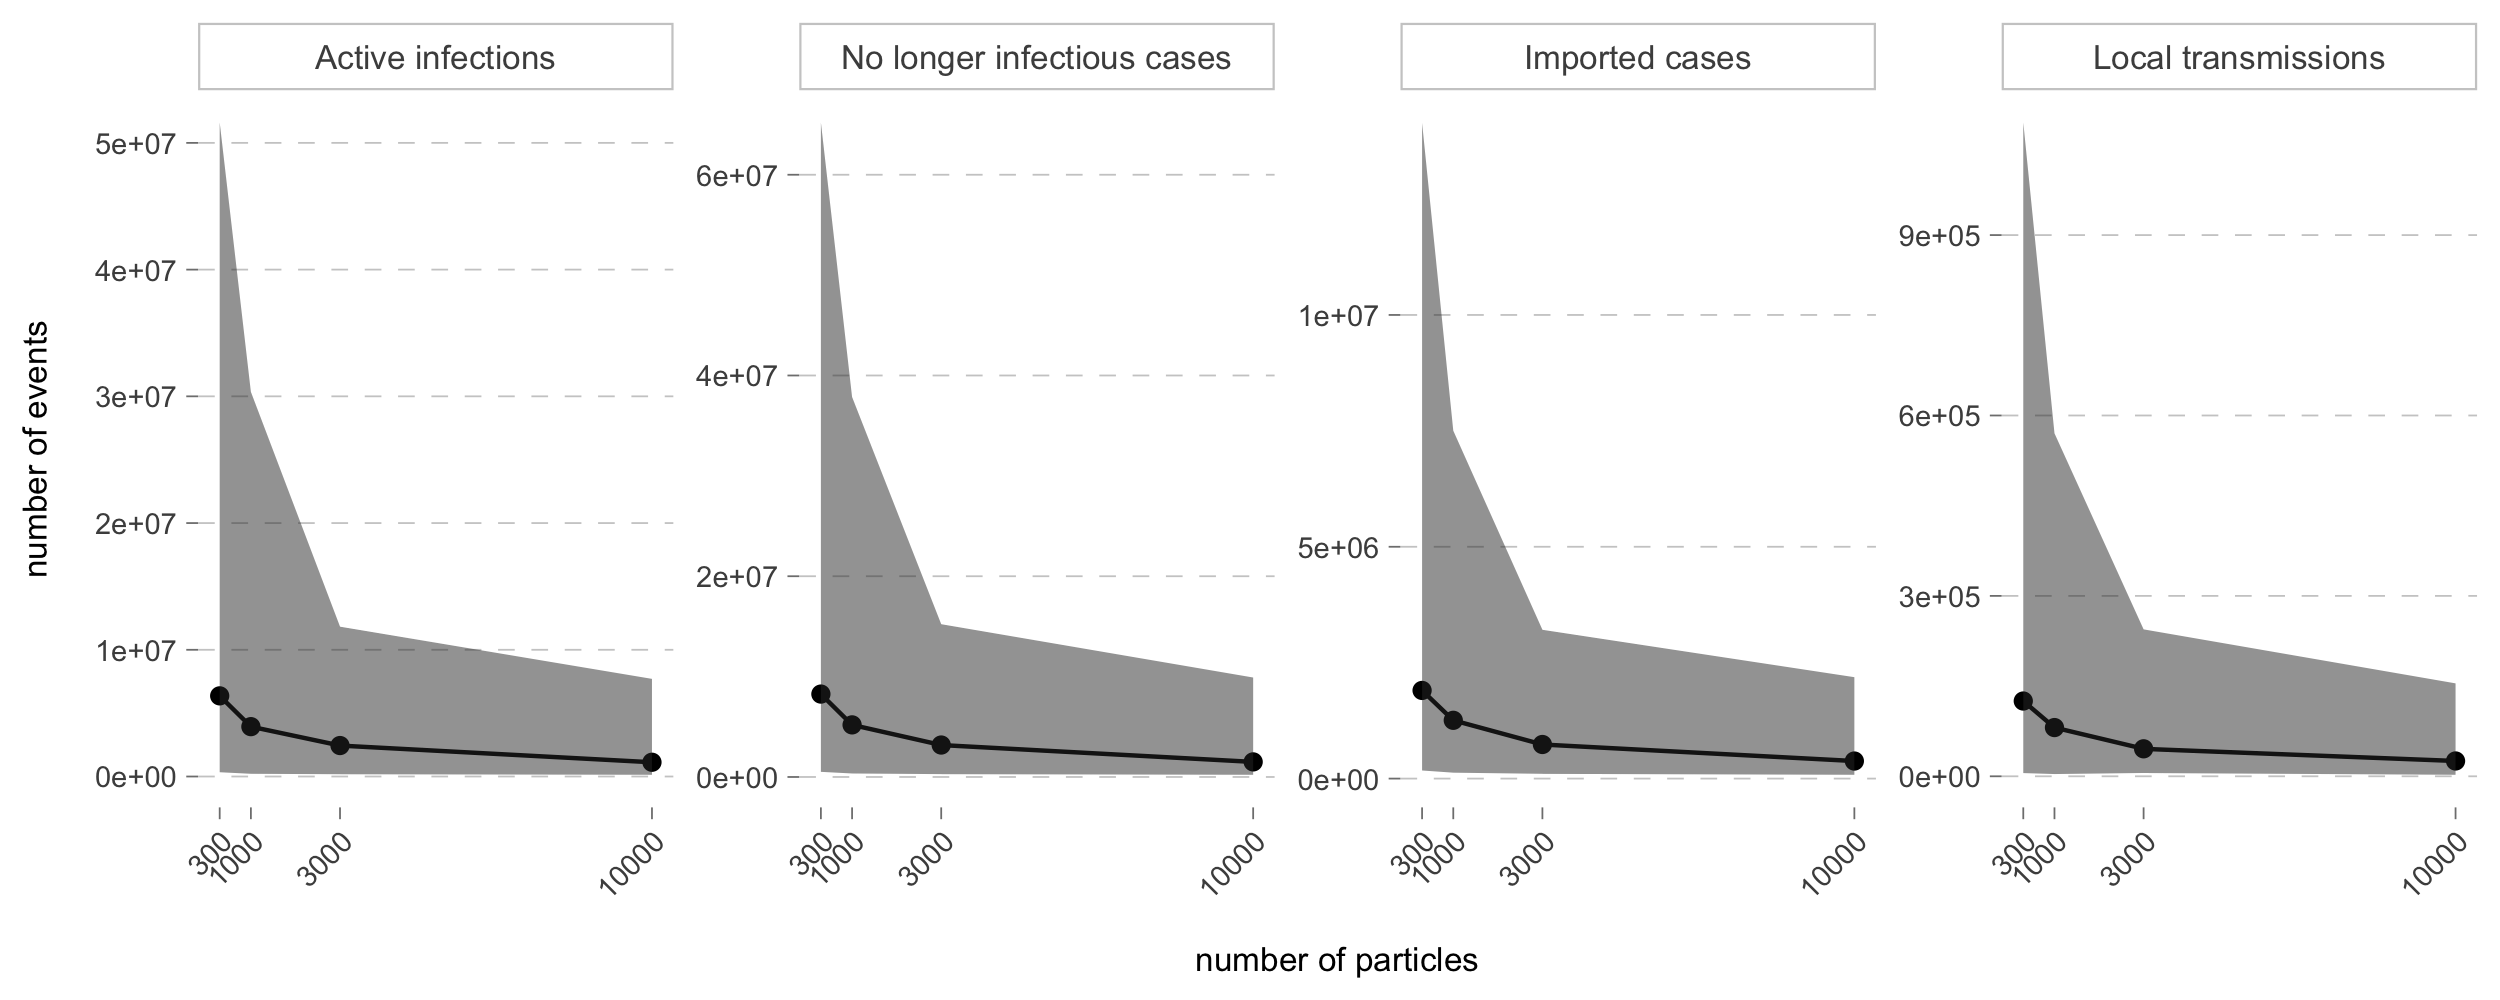
\includegraphics[width=\textwidth]{particles_comparison.png}
    \caption{First introductions of SARS-CoV-2. From the set of random subsampled trajectories, the first introduction time for each epidemic trajectory is recorded and the probability distribution over all these times is plotted. \textbf{A} Probability density of the time of first introduction for each deme. Each dotted line represents the first date when cases where reported to ECDC by deme color. In the case of China, the distribution of the origin time is plotted, since in the analysis we defined Chine as the origin of the epidemic with probability 1. For the other five demes, the distribution of the time of first migration into the deme is shown. \textbf{B} Stacked probability density of the destination of first introduction into Europe coloured by the destination deme. This first case corresponds to the first migration event from China to any of the European countries. \textbf{C} Stacked probability density of the source of the first introduction for each deme coloured by the source deme of the introduction.}
    \label{fig:particles}
    \todo[inline]{ticks for every month}
\end{figure}